%%%%%%%%%%%%%%%%%%%%%%%%%%%%%%%%%%%%%%%%%
% Thin Sectioned Essay
% LaTeX Template
% Version 1.0 (3/8/13)
%
% This template has been downloaded from:
% http://www.LaTeXTemplates.com
%
% Original Author:
% Nicolas Diaz (nsdiaz@uc.cl) with extensive modifications by:
% Vel (vel@latextemplates.com)
%
% License:
% CC BY-NC-SA 3.0 (http://creativecommons.org/licenses/by-nc-sa/3.0/)
%
%%%%%%%%%%%%%%%%%%%%%%%%%%%%%%%%%%%%%%%%%

%----------------------------------------------------------------------------------------
%	PACKAGES AND OTHER DOCUMENT CONFIGURATIONS
%----------------------------------------------------------------------------------------

\documentclass[a4paper, 11pt]{article} % Font size (can be 10pt, 11pt or 12pt) and paper size (remove a4paper for US letter paper)

\usepackage[protrusion=true,expansion=true]{microtype} % Better typography
\usepackage{graphicx} % Required for including pictures
\usepackage{wrapfig} % Allows in-line images
\usepackage{amsmath,amssymb}

\usepackage[tikz]{bclogo}

\usepackage{mathpazo} % Use the Palatino font
\usepackage[T1]{fontenc} % Required for accented characters
\linespread{1.1} % Change line spacing here, Palatino benefits from a slight increase by default

\makeatletter
%\renewcommand\@biblabel[1]{\textbf{#1.}} % Change the square brackets for each bibliography item from '[1]' to '1.'
\renewcommand{\@listI}{\itemsep=0pt} % Reduce the space between items in the itemize and enumerate environments and the bibliography

\renewcommand{\maketitle}{ % Customize the title - do not edit title and author name here, see the TITLE block below
\begin{flushright} % Right align
{\LARGE\@title} % Increase the font size of the title

\vspace{50pt} % Some vertical space between the title and author name

{\large\@author} % Author name
\\\@date % Date

\vspace{40pt} % Some vertical space between the author block and abstract
\end{flushright}
}


%----------------------------------------------------------------------------------------

\begin{document}


\tableofcontents
\newpage
%----------------------------------------------------------------------------------------
%	ESSAY BODY
%----------------------------------------------------------------------------------------
\section{Hierarchy}
Space and time are the two basic properties used to organize perceptions of the world around us. Real world events unfold over a wide range of length and time scales. A strategy the the brain has developed to make sense of these perception is a hierarchy in processing of information. -- check, rewrite --

Visual information enters the brain in the primary visual cortex.
Ungerleider and Mishkin \cite{mishkin1983object} put forward evidence for a two distinct cortical visual pathways, the ventral and dorsal pathway, which go through the temporal and parietal cortex, respectively; see figure \ref{fig:visualpathways}. 
\begin{figure}[!ht]
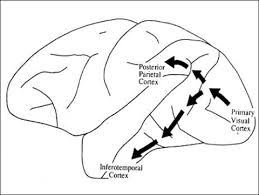
\includegraphics[scale=1]{hierarchy_figures/visualpathways}
\caption{find better image!!!}
\label{fig:visualpathways}
\end{figure}
The distinction is made on basis of the function: the ventral pathway is specialized in determining what an object is, and the dorsal pathway in determining the location of an object.
A later study, by  Milner and Goodale \cite{milner2008two, goodale1992separate}, found the same two pathways; however, they characterized the pathways in a different manner. They concluded that the ventral stream is specialized in perception and the dorsal stream in action.
The ventral and dorsal pathways exist in other sensory systems as well.

\subsection{Processing hierarchy}

One of the fundamental organizational principles of the visual system in brain is the increase in the size of the spatial receptive field (SRF) along the a cortical visual pathway \cite{hubel1988eye,hubel1962receptive,lerner2001hierarchical}.
In the primary visual cortex,  the starting point of the visual pathway, the SRF is small.
Further along the visual pathway neurons receive input from an increasing number of neurons, each with a smaller SRF. This results in integration of stimuli over a larger space, which enables brain functions such as size invariant object recognition \cite{kobatake1994neuronal}.

Recent experimental research, inspired by the SRF, has shown the a similar hierarchy exists in the processing time scale in the brain \cite{hasson2008hierarchy, lerner2011topographic, honey2012slow}.
Lerner et al. used a scrambled story to show the existence of a temporal hierarchy \cite{lerner2011topographic}.
As a measure for the timescale the temporal receptive window (TRW) is defined as the length of time before a response during which sensory information may affect that response.
The TRW is the homologue of the SRF in the spatial hierarchy. 
The TRWs of different brain areas was determined by measuring the reliability of neural responses, in human subjects, as a result of listening to a narrated story of seven minutes.
This story was played 4 times, each time scrambled on  different timescale.
In the short timescale story the words of the story were scrambled (segments of $1 \pm 0.5 s$).
In the intermediate scrambled story the sentences were scrambled (segments of $7 \pm 3 s$). For the long timescale story the paragraphs were scrambled (segment of $38 \pm 17 s$).
For the story with the shortest timescale the story was played backwards (coherent on $<1 s$ timescale).
By comparing the reliability of different neuronal responses to the scrambled stories one is able to characterize one of the computational properties of a brain area, i.e. the TRW.
The neuronal responses were measured using fMRI BOLD analysis (see appendix \ref{app:A}.
The reliability of a response was determined by intersubject correlation analysis: comparing the BOLD signal response time courses across different subjects using the Pearson correlation coefficient
\begin{equation}\label{eq:intersubject_corrrelation}
\rho_k = \rho(r_k,\bar{r}) = \frac{r_k(t) \cdot \bar{r}(t)}{•\sqrt{(r_k(t) \cdot r_k(t))(\bar{r}(t) \cdot \bar{r} (t))}},
\end{equation}
with $r_k(t)$ the mean-subtracted response time course of a voxel of subject k.
The mean response, $\bar{r}(t)=\sum_{i\neq k} r_i(t)$ , is the response time course averaged over all subjects except subject k.
The dots represents inner products.
The results from the intersubject analysis is shown in figure \ref{fig:timescale_hierarchy}.

\begin{figure}[!ht]
\centering
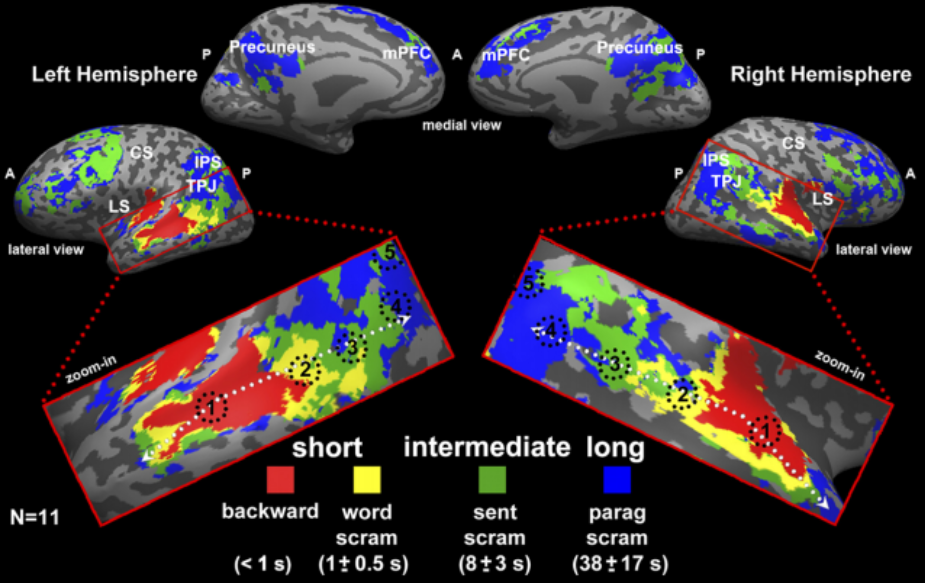
\includegraphics[scale=0.38]{hierarchy_figures/temporal_hierarchy}
\caption{
The results from the intersubject analysis. 
A voxel was colored red if the voxel has a significant correlation coefficient (eq. \ref{eq:intersubject_corrrelation}) for all types of stories.
A voxel was colored yellow if it has a significant correlation coefficient for all stories except backwards played story.
The green voxels correspond to voxels with a significant correlation coefficient for all types of stories except the backwards played and word scrambled stories.
A green voxel corresponds to a voxel with a significant correlation coefficient only for the paragraph scrambled story.
The correlation coefficient of a voxel is deemed significant if the coefficient is above a certain value for all subjects (for details see \cite{lerner2011topographic}).
The circled numbers are positioned along the A1-TPJ axis. With 1 indicating A1 an early area and 5 TPJ (the temporal-perietal junction) a higher order area.
A and P indicate respectively the anterior and posterior of the brain.
Figure taken from \cite{lerner2011topographic}. }
\label{fig:timescale_hierarchy}
\end{figure}

These results show that the reliability of the neuronal response in different brain areas varies as the temporal structure of the information is modified.
The response reliability in early auditory areas is not affected by changing the temporal structure of the story.
Higher order auditory brain areas have a increased neuronal response reliability as the temporal structure of the stimulus is increased.
Previously, a similar study has been done, also using fMRI BOLD analysis, but with a silent movie instead of a narrated story \cite{hasson2008hierarchy}.
Combining the results from the narrated story and the movie suggests that the structure in the hierarchy of the TRWs is a general organizational principle in the human cortex; see figure \ref{fig:timescale_hierarchy_story_movie}.
The early visual and auditory area have short TRWs, and the TRWs increase as one move to higher order areas. Some higher order areas  have a  mutlimodal TRW, as they process long temporal structures, whether presented aurally or visually.


\begin{figure}[!ht]
\centering
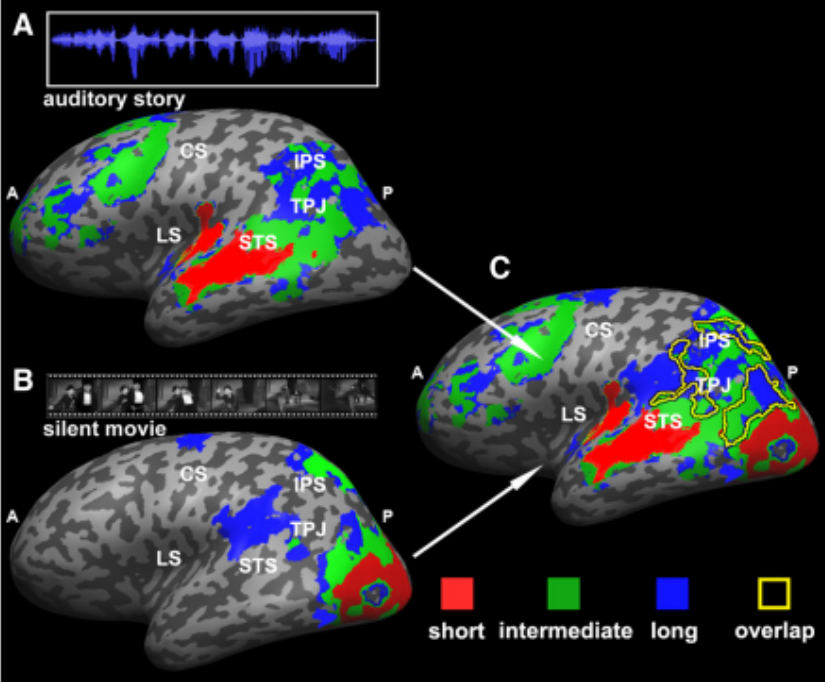
\includegraphics[scale=0.38]{hierarchy_figures/temporal_hierarchy_story_movie}
\caption{
TRW hierarchy as a general topographic organizational principle of the human cortex.
(A) The response reliability of the scrambled narrated story. (B) The response reliability of the silent movie. (C) Superposition of both response reliabilities. 
Figure taken from \cite{lerner2011topographic}.
}
\label{fig:timescale_hierarchy_story_movie}
\end{figure}
Recently a similar study has been done with a scrambled movie with sound, but using ECoG in stead of fMRI BOLD recording \cite{honey2012slow}. The results from that study corroborated the conclusion from Hasson et al. and Lerner et al. that there exists a ordered topographic hierarchy in the TRWs of brain areas \cite{lerner2011topographic, hasson2008hierarchy}.
In addition Honey et al. showed that slow components of neuronal dynamics are more prominent in regions with longer TRWs compared with regions with shorter TRWs, and that regions with a longer TRW exhibit a greater temporal autocorrelation than regions with a shorter TRW.
These findings are consistent with the hypothesis that early sensory brain areas, with a short TRW, are optimized for tracking rapid response to the input, and that, on the other hand, higher order areas, which have a longer TRW, accumulate information over time \cite{huk2005neural, ogawa2010differential, romo1999neuronal, shadlen2001neural, wang2002probabilistic}.
A longer TRW is useful for perceptual and cognitive tasks such as segmenting ongoing activity in temporal parts \cite{zacks2001human,hasson2008hierarchy}, short-term memory \cite{hasson2015hierarchical, durstewitz2000neurocomputational}, inference of cause and effect \cite{fonlupt2003perception}, and processing language with a wide variety of time scales (e.g. complete narrative, paragraph, sentence, and words) \cite{xu2005language, lerner2011topographic}.
Lerner et al. found that the TRWs of the brain areas rescale, up to a certain limit, when the incoming rate of information is changed \cite{lerner2014temporal}.
A similar phenomenon is also observed in the change in SRF size \cite{sheinberg2001noticing, furmanski2004learning, moran1985selective}.
Though the rate of incoming information can modulate the TRWs, the time scale gradient is an intrinsic property of neural circuits \cite{stephens2013place}.

-- why is ecog important -- 


\subsection{ A large-scale dynamical model}

Recently Chaudhuri et al. developed a large-scale dynamical model of the macaque neocortex \cite{chaudhuri2015large-scale}.
The model is based on recently acquired connectivity from tract tracing experiment \cite{markov2012weighted, markov2014anatomy}. Previously Markov et al. and Ercsey-Ravasz et al. 
The connectivity is strength is characterized by the fraction of labeled neurons (FLN); the FLN from area B to A is defined as:
\begin{equation}
FLN_{B\rightarrow A} = \frac{number\ of\ neurons\ projecting\ from\ B\ to\ A}{total\ number\ of\ neurons\ projecting\ to\ A}.
\end{equation}
The counting of the projecting neurons is done using retrograde tracer injections. For further details on the data acquisition see refs. \cite{markov2012weighted, markov2014anatomy, markov2011weight, kennedy2013data}. 
Not all FLN values between all brain areas of the macaque neocortex are know; therefore only a subnetwork of 29 areas, of which all FLN values are known, is used.
In addition to the FLN values, the fraction of supragranular layer neurons (SLN) is know of all connections between the areas. The SLN from area B to A is defined as
\begin{equation}
SLN_{B\rightarrow A} = \frac{number\ of\ supragranular\ neurons\ projecting\ from\ B\ to\ A}{number\ of\ neurons\ projecting\ from\ B\ to\ A}.
\end{equation}

Neurons mediating feedforward projections originate mostly from the supragranular layers.
Feedback projections, on the other hand, are primarily mediated by neurons originating from the infragranular layers of the cortex \cite{felleman1991distributed}. So if the connection from area A to B is mostly feedforward (feedback) $0.5 < SLN_{A\rightarrow B} < 1$ ($0 < SLN_{A\rightarrow B} <0.5$).
See appendix \ref{app:B} for information on cortical layers.
Using the SLN one can order the 29 brain areas such that the first area receives mostly feedback projections and its output is primarily feedforward, and the last area the other way around.
The hierarchical position can be quantified by assigning a number $h\in (0,1]$ each area \cite{chaudhuri2015large-scale, markov2014anatomy}.
The hierarchical position correlates to basal dentritic spine count. Spines are places were a other neuron can attach to. These  increase sharply from primary sensory areas to prefrontal areas.
Because this connections are primarily excitatory -- find ref -- the spine count is used as a proxy for excitatory connection strength, a gradient in the excitatory connection strength is introduced in the model \cite{elston2000pyramidal,elston2011pyramidal}.
Previously Chaudhuri et al. showed, using a simpler network architecture, that introducing a gradient in the connection strength leads to localized eigenvectors with a gradient in time constants \cite{chaudhuri2014diversity}.
To study the dynamics a threshold linear model was used, where each area is modeled as a single node which exists in an excitatory and an inhibitory version.
The resulting  network has 58 nodes. 
The time-evolution -- check -- of the firing rates of the nodes in the inhibitory and excitatory population, $\nu_I$ and $\nu_E$ respectively, are governed by the following equations,
\begin{multline}
\label{eq:wang_exc}
\tau_E \frac{d}{dt} \nu_E^i = - \nu_E^i + \\ \beta_E \left[ \left( 1+\eta h_i \right) \left( w_{EE} \nu_E^i + \mu_{EE} \sum_{j=1}^N FLN_{ij} \nu_E^j \right) - w_{EI} \nu_I^i+ I_{ext,E}^i \right]_+,
\end{multline}

\begin{multline}
\label{eq:wang_inh}
\tau_I \frac{d}{dt} \nu_I^i =  - \nu_I^i + \\  \beta_I \left[ \left( 1+\eta h_i \right) \left( w_{IE} \nu_E^i + \mu_{IE} \sum_{j=1}^N FLN_{ij} \nu_E^j \right) - w_{II} \nu_I^i+ I_{ext,I}^i \right]_+,
\end{multline}
with
\begin{equation*}
\left[x \right]_+ = \begin{cases}
	x, & \text{if } x>0\\
	0, & \text{if } x\leq0.
	\end{cases}
\end{equation*}
The parameter $\eta$ controls the effect of the gradient in the excitatory connection strength; $i$ and $j$ are the indices of the nodes; the hierarchical position of each node is $h_i$; $I_{ext,E}^i$ and $I_{ext,E}^i$ are the external inputs to node $i$ of the excitatory and inhibitory node, respectively.
All the other values of the parameters are taken from ref. \cite{binzegger2009topology}.

\begin{figure}[!ht]
\centering
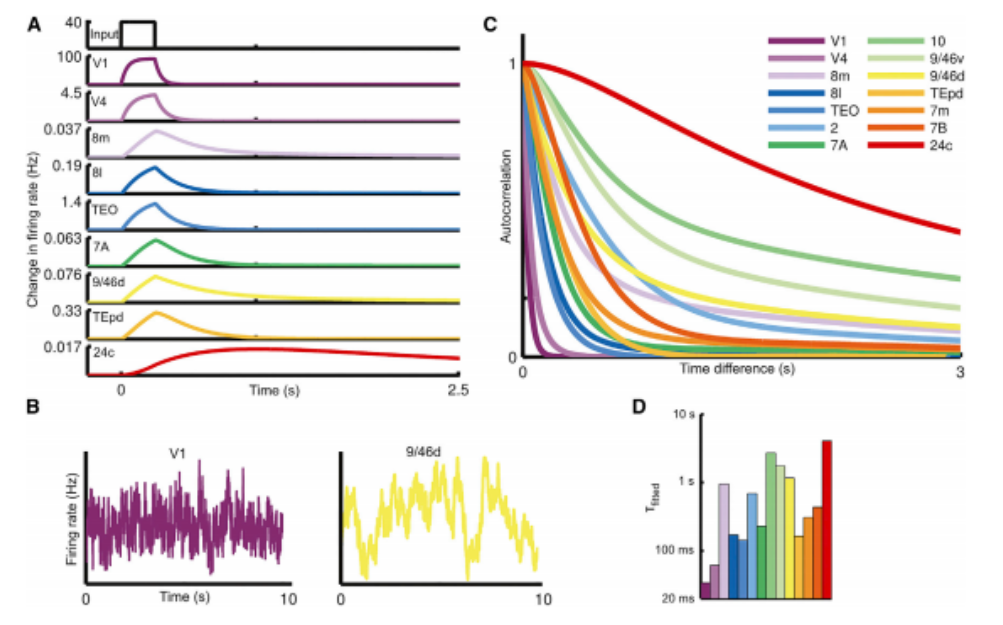
\includegraphics[scale=0.3]{wang_figures/mainfig}
\caption{A hierarchy of time scales in response to visual input.
(A) A pulse input to V1 in the primary visual cortex. Early areas can track the input with greater accuracy than latter areas, where the affect of the pulse persist for a longer period of time. The areas are ordered from earliest area, V1, in the hierarchy on top and the last area in the hierarchy, 25c, on the bottom.
(B) The response of areas V1 and 9/46d to white noise input to area V1.
(C) The autocorrelation of 14 areas decay over a wide range of time scales.
(D) The fitted time constants to the autocorrelations in (C). A trend is clearly visible: time constants increase along the hierarchy. Ordered from earliest area in the hierarchy, V1, on the left to the last area in the hierarchy, 25c, on the right.
Figure taken from \cite{chaudhuri2015large-scale}.
}
\label{fig:wang_fig}
\end{figure}

The response of the nodes in the network to pulsed input to area V1, in the primary visual cortex, is shown in figure \ref{fig:wang_fig} A. Early areas such as V1 and V4 can track the pulse with greater accuracy than latter areas; e.g., 24c where the response to the pulse is smeared out over several seconds.
As a measure for the time constant of each area the decay time of the autocorrelation of the response to white noise input to area V1 are used \ref{fig:wang_fig} B and C.
The decay time of the areas tend to increase along the hierarchy \ref{fig:wang_fig} D.
Though a trend is apparent, the time scales do not increase monotonously along the hierarchy. 

\begin{figure}[!ht]
\centering
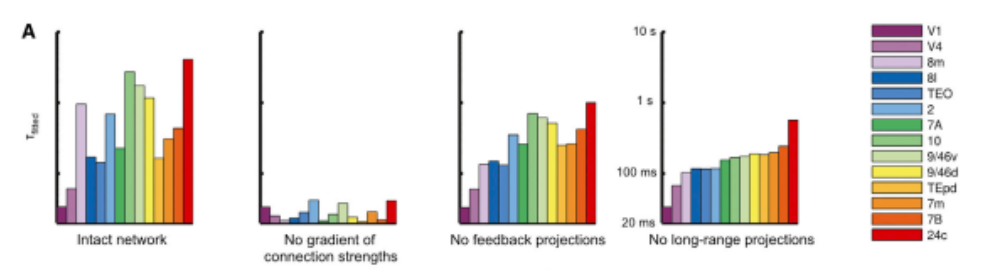
\includegraphics[scale=0.3]{wang_figures/time_consts}
\caption{The timescales for different models. Far left: the intact network. Second from the left: the model without the gradient in excitatory connection strength; i.e., $\eta=0$ in eqns. \ref{eq:wang_exc} and \ref{eq:wang_inh}. The trend in the time constants is destroyed, and all time constants are decreased significantly, mostly in area further in the hierarchy.
Third from the left: the time constants of the areas with the feedback projections removed. The decrease of the time constants in the areas higher up in the hierarchy shows the tendency of these areas to form feedback loops.
Far right: the network without long-range projections. In this network the time constants follow the same order as the hierarchy.
Figure taken from \cite{chaudhuri2015large-scale}.
}
\label{fig:wang_time_consts}
\end{figure}

In order to show that the gradient in the connection strength is indeed the origin of the gradient in the time scales  different aspects of the model are removed; see figure \ref{fig:wang_time_consts}.
Removing the hierarchy in excitatory connection strength destroys the trend in the time scales; there is no longer a a relation ship between the position in the hierarchy and the time scale of the area.
This is a result from  the decrease in time scales of areas further along the hierarchy.
Removing the feedback projections, determined by the SLN value \cite{felleman1991distributed}, from the connectivity matrix results in a decrease in the range of the time scales, showing that slow areas tend to form excitatory loops.
Without long-range projections, e.i. setting all $FLN_{ij}=0$ for all $i$ and $j$, the order of the areas is the same when the areas are ordered by time constant or hierarchical position.

\begin{figure}[!ht]
\centering
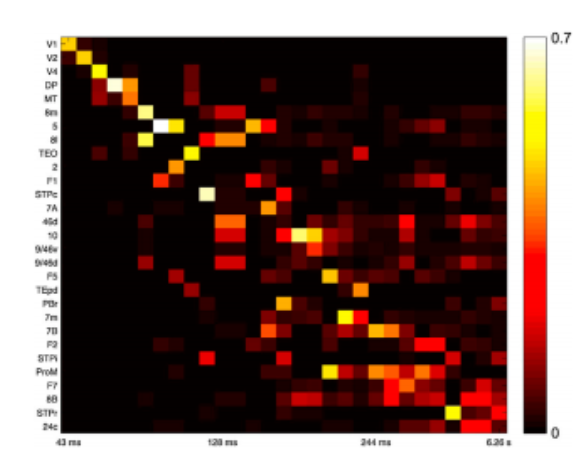
\includegraphics[scale=0.4]{wang_figures/eigenvecs}
\caption{ The eigenvectors of the linearized equations. The eigenvectors are represented by the columns. The area corresponding to the entry of the eigenvector are shown on the left, ordered by hierarchical position with the first area on top.
Figure taken from \cite{chaudhuri2015large-scale}.
}
\label{fig:wang_eigenvecs}
\end{figure}

Neglecting the non-linearity in the model, replacing $[x]_+$ by  $[x]=x$ in eqns. \ref{eq:wang_exc} and \ref{eq:wang_inh}, one can use linear system analysis. In a linear system the activity is the weighted sum of the eigenvectors \cite{rugh1993linear}. The timescales of the eigenvector are given by $\tau = 1/Re\{\lambda\}$. The eigenvectors of the linearized model are localized, in the sense that each eigenvector has a significant amplitude in only a small number of entries \ref{fig:wang_eigenvecs}. The eigenvectors that are localized in the areas early in the hierarchy have a short time scale ($~43 ms$), and the last areas in the hierarchy have a timescale that is larger by several orders of magnitude ($~6 s$). This corroborates the findings in figure \ref{fig:wang_fig}: areas early in the hierarchy have a short time scale and areas further up in the hierarchy have an increasingly longer timescale.


\section{Balance}


-- criticality --
-- random matriced  -- 






\newpage
\section{Appendix A}\label{app:A}
Explain fMRI, BOLD and ecog.

\newpage
\section{Appendix B}\label{app:B}
Explain cortical collumns and layers

%----------------------------------------------------------------------------------------
%	BIBLIOGRAPHY
%----------------------------------------------------------------------------------------
\newpage
\addcontentsline{toc}{section}{References}
\bibliographystyle{unsrt}

\bibliography{bibliography}

%----------------------------------------------------------------------------------------

\end{document}
